\chapter{Аналитический раздел}
В данном разделе будут рассмотрены теоретические основы работы алгоритмов поиска значения в словаре по ключу.

\section{Понятие словаря}
Словарь - это структура данных, представляющая из себя ассоциативный массив, позволяющий хранить пары вида ключ-значение. Операции, которые поддерживает словарь, включают в себя добавление пары, удаление пары по ключу, поиск пары по ключу. Также в словарях не может быть двух пар с одинаковыми ключами. 

На данный момент существует множество вариантов поиска в словаре по ключу. В этой лабораторной работе будут рассмотрены следующие алгоритмы:
\begin{itemize}
	\item поиск полным перебором;
	\item двоичный поиск в упорядоченном словаре;
	\item частичный анализ для поиска в словаре.
\end{itemize}

\section{Алгоритм полного перебора}
Алгоритм полного перебора подразумевает последовательный проход по словарю, в процессе которого каждый ключ из каждой пары сравнивается с искомым ключом, пока не будет найдено совпадение. Лучшим случаем для данного алгоритма является ситуация, когда искомый ключ находится в начале словаря, в результате происходит одно сравнения. Худших случаев два - ключ не найден и ключ находится в конце. 

\section{Алгоритм двоичного поиска в упорядоченном словаре}
Двоичный поиск использует отсортированный массив ключей. Идея заключается в выделении среднего для фрагмента элемента и сравнения ключа с ним. Так как список отсортирован, мы можем с лёгкостью определять при каждом сравнении, в какой половине фрагмента находится элемент, пока не дойдём до самого элемента. Лучший случай алгоритма - элемент находится в центре, в следствие чего находится за один прогон цикла. Худшим случаем является нахождение элемента на краях массива, в начале или в конце. Так как длина части, в которой мы ищем элемент, каждый раз сокращается в два раза, то общая сложность будет задаваться как $O(log_{2}n)$.

\section{Алгоритм частичного анализа для поиска в словаре}
Использование частичного анализа подразумевает, что словарь, подающийся на вход, был отсортирован по частоте встречаемости первого символа каждого ключа словаря. Ключами нового словаря являются буквы алфавита. Новый словарь формируется таким образом, что первая буква ключей основного словаря совпадается с ключами нового словаря в результате чего такая организация напоминает толковый словарь. Изначально поиск ведётся по первой букве, а затем полным перебором. В худшем случае первая буква у всех ключей будет одна и та же, что приведёт к тому, что алгоритм будет работать, как алгоритм полного перебора. В лучшем случае ключ в новом словаре будет указывать на словарь из одного слова, которое и является искомым ключом.

\section{Вывод}
В данном разделе были рассмотрены основные теоретические сведения об алгоритмах полного перебора, бинарного поиска и частичного анализа. В результате были сделаны выводы о том, что на вход алгоритму подаётся словарь и искомый ключ, а на выходе программа возвращает значение, которое соответствует данному ключу. Алгоритмы работают на словарях размероностью от 0 до физически возможного предела для используемой машины. В качестве критерия для сравнения эффективности алгоритмов будет использоваться время работы на словарях различных размерностей.

\chapter{Конструкторский раздел}

В данном разделе будут рассмотрены схемы, структуры данных, способы тестирования, описания памяти для следующих алгоритмов:
\begin{itemize}
	\item алгоритм полного перебора;
	\item алгоритм бинарного поиска;
	\item алгоритм частичного анализа.
\end{itemize}

\section{Тестирование алгоритмов}

Описание тестов:
\begin{enumerate}
	\item проверка работы на ключе из начала словаря;
	\item проверка работы на ключе из середины словаря;
	\item проверка работы на ключе из конца словаря;
	\item проверка работы на несуществующем ключе.
\end{enumerate}

\section{Алгоритм полного перебора}

Используемые типы и структуры данных включают в себя:
\begin{enumerate}
	\item integer, целое число - используется для хранения индексов массива, размера массива;
	\item dict, словарь - стандартная структура данных, использующаяся для хранения словаря.
\end{enumerate}

\newpage

\begin{figure}[ph!]
	\center{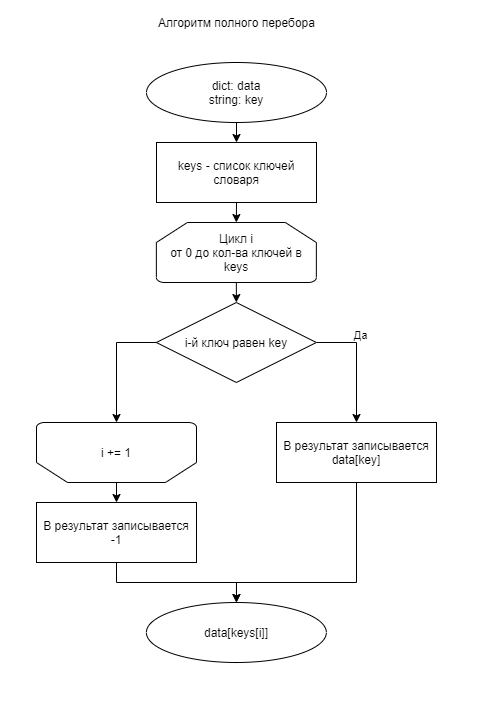
\includegraphics[scale=0.7]{brute_force_scheme}}
	\caption{Схема алгоритма полного перебора}
\end{figure}

\section{Алгоритм бинарного поиска}

Используемые типы и структуры данных включают в себя:
\begin{enumerate}
	\item integer, целое число - используется для хранения индексов массива, размера массива;
	\item dict, словарь - стандартная структура данных, использующаяся для хранения словаря.
\end{enumerate}


\begin{figure}[ph!]
	\center{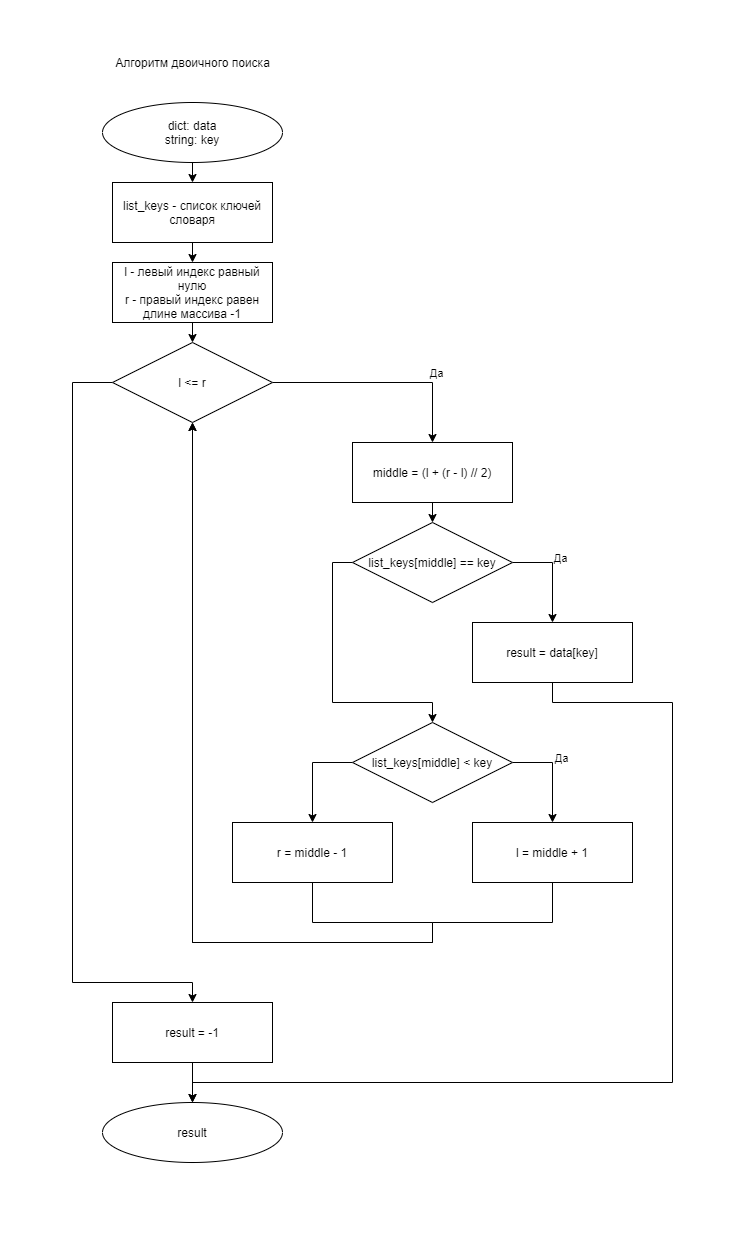
\includegraphics[scale=0.7]{bin_scheme}}
	\caption{Схема алгоритма бинарного поиска}
\end{figure}

\newpage

\section{Алгоритм частичного анализа}

Используемые типы и структуры данных включают в себя:
\begin{enumerate}
	\item integer, целое число - используется для хранения индексов массива, размера массива;
	\item dict, словарь - стандартная структура данных, использующаяся для хранения словаря.
\end{enumerate}


\begin{figure}[ph!]
	\center{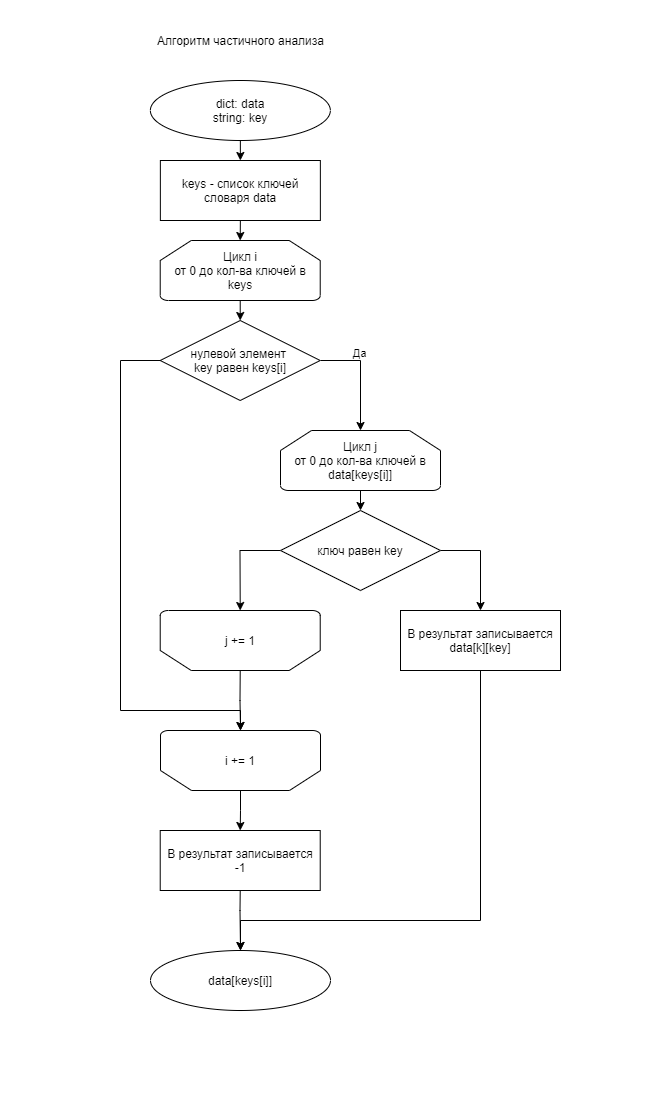
\includegraphics[scale=0.7]{seg_scheme}}
	\caption{Схема алгоритма частичного анализа}
\end{figure}

\newpage

\section{Функциональная схема ПО}
На изображении ниже представлена функиональная схема разрабатываемого ПО. На вход подаётся словарь и ключ, при помощи алгоритмов, реализованных на языке Python мы получаем в результате работы значение, соответствующее ключу.

\begin{figure}[ph!]
	\center{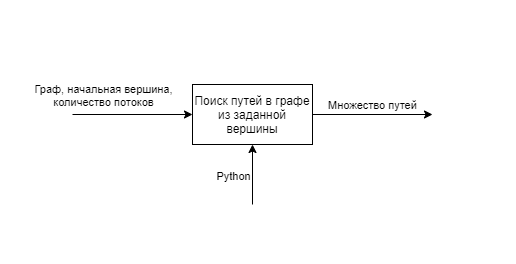
\includegraphics[scale=1.0]{func_scheme}}
	\caption{IDEF0 диаграмма разрабатываемой программы}
\end{figure}

\section{Вывод}
В данном разделе были рассмотрены схемы алгоритмов полного перебора, бинарного поиска и частичного анализа. Были определены тесты для каждого алгоритма и описаны типы и структуры данных, использующихся в алгоритмах. Также была приведена функциональная схема разрабатываемого ПО.

\chapter{Технологический раздел}

В данном разделе будут рассмотрены подробности реализации описаных выше алгоритмов. Также будут обоснованы выбор языка программирования для реализации, выбор библиотек для проведения экспериментов и представлены важные фрагменты кода написанной в рамках работы программы.

\section{Выбор языка программирования}

В качестве языка программирования для реализации данной лабораторной работы использовался язык программирования Python поскольку он предоставляет широкие возможности для эффективной реализации алгоритмов. В качестве среды разработки использовалась Visual Studio Code по причине того, что данная среда имеет встроенные средства отладки и анализа работы программы, позволяющие быстро и эффективно писать код.

\section{Сведения о модулях программы}

Реализованное ПО состоит из трёх модулей:
\begin{enumerate}
	\item main - основной файл программы, где находится точка входа;
	\item tests - реализация тестов алгоритмов;
	\item algos - реалиазция алгоритмов.
\end{enumerate}

\section{Реализация алгоритмов}

\begin{lstlisting}[label=some-code-1,caption=Реализация алгоритма полного перебора]
def seq_search(data, key):
    for elem in data:
        if key == elem:
            return data[elem]
    return -1
\end{lstlisting}

\begin{lstlisting}[label=some-code-2,caption=Реализация алгоритма бинарного поиска]
def bin_search(data, key):
    list_keys = sorted(list(data.keys()))
    l, r = 0, len(list_keys) - 1
    while l <= r:
        middle = (l + (r - l) // 2)

        if list_keys[middle] == key:
            return data[key]
        elif list_keys[middle] < key:
            l = middle + 1
        else:
            r = middle - 1

    return -1
\end{lstlisting}

\begin{lstlisting}[label=some-code-3,caption=Реализация алгоритма частичного анализа]
def seg_search(data, key):
    for k in data:
        if key[0] == k:
            for elem in data[k]:
                if elem == key:
                    return data[k][elem]
    return -1
\end{lstlisting}

\section{Результаты тестирования алгоритмов}

Для тестирования алгоритмов было реализованы следующие тесты:
\begin{enumerate}
	\item проверка работы на ключе из начала словаря;
	\item проверка работы на ключе из середины словаря;
	\item проверка работы на ключе из конца словаря;
	\item проверка работы на несуществующем ключе.
\end{enumerate}

Результаты тестов:
\begin{figure}[ph!]
	\center{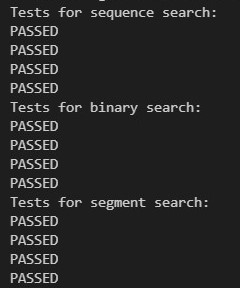
\includegraphics[scale=1.0]{test_results}}
	\caption{Результаты тестирования алгоритмов}
\end{figure}

\section{Вывод}
В данной разделе были представлены реализации алгоритма полного перебора, бинарного поиска и частичного анализа, а также представлены результаты работы модуля тестирования реализованных алгоритмов.

\chapter{Экспериментальный раздел}

В данном разделе описываются измерения временных характеристики алгоритмов полного перебра, бинарного поиска и частичного анализа для различных положений ключа в словаре, а также делается вывод об эффективности алгоритмов для соответствующих случаев.

\section{Технические характеристики}
\begin{itemize}
	\item Операционная система - Windows 10, 64-bit;
	\item Оперативная память - 16 GiB;
	\item Процессор - Intel(R) Core(TM) i7-9750H CPU @ 2.60GHz 2.59 GHz, 6 ядер, 12 потоков.
\end{itemize}

\section{Результаты экспериментов}

\newpage
\subsection{Результаты экспериментов для ключа в начале словаря}

\begin{table}[ph!]
  \begin{center}
    \captionsetup{justification=raggedright}
     \caption{Время работы алгоритмов при предварительной сортировке с ключом в начале}
    \label{tab:workcost_classic}
    \begin{tabular}{c|c|c|c}
      \textbf{кол-во пар} & \textbf{t полного перебора (нс)}  & \textbf{t бинарного поиска (нс)} & \textbf{t частичного анализа (нс)}\\
	100000 & 0 & 0 & 0\\
	150000 & 0 & 0 & 0\\       
	200000 & 0 & 0 & 0\\       
	250000 & 0 & 0 & 3125000\\ 
	300000 & 0 & 0 & 0\\       
	350000 & 0 & 0 & 0\\       
	400000 & 0 & 0 & 0\\       
	450000 & 0 & 0 & 0\\       
	500000 & 0 & 0 & 0\\ 
      \hline	
    \end{tabular}
  \end{center}
\end{table}

\begin{figure}[ph!]
	\center{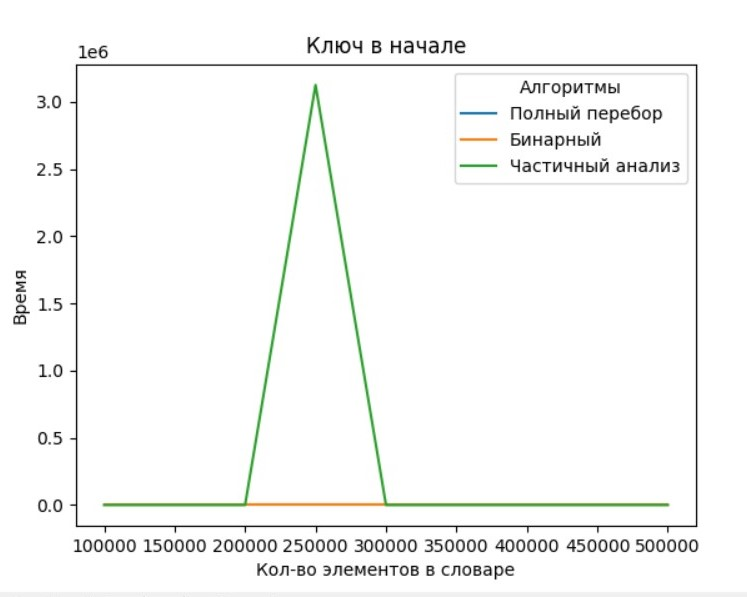
\includegraphics[scale=0.7]{res_start_presort}}
	\caption{График зависимости времени работы от размерности словарей при предварительной сортировке с ключом в начале}
\end{figure}

\newpage
\begin{table}[ph!]
  \begin{center}
    \captionsetup{justification=raggedright}
     \caption{Время работы алгоритмов без предварительной сортировки с ключом в начале}
    \label{tab:workcost_classic}
    \begin{tabular}{c|c|c|c}
      \textbf{кол-во пар} & \textbf{t полного перебора (нс)}  & \textbf{t бинарного поиска (нс)} & \textbf{t частичного анализа (нс)}\\
	100000 & 0 & 78125000 & 62500000\\
	150000 & 0 & 134375000 & 96875000\\
	200000 & 0 & 187500000 & 137500000\\
	250000 & 0 & 246875000 & 187500000\\
	300000 & 0 & 312500000 & 218750000\\
	350000 & 0 & 425000000 & 265625000\\
	400000 & 0 & 450000000 & 296875000\\
	450000 & 0 & 537500000 & 340625000\\
	500000 & 0 & 584375000 & 415625000\\
      \hline	
    \end{tabular}
  \end{center}
\end{table}

\begin{figure}[ph!]
	\center{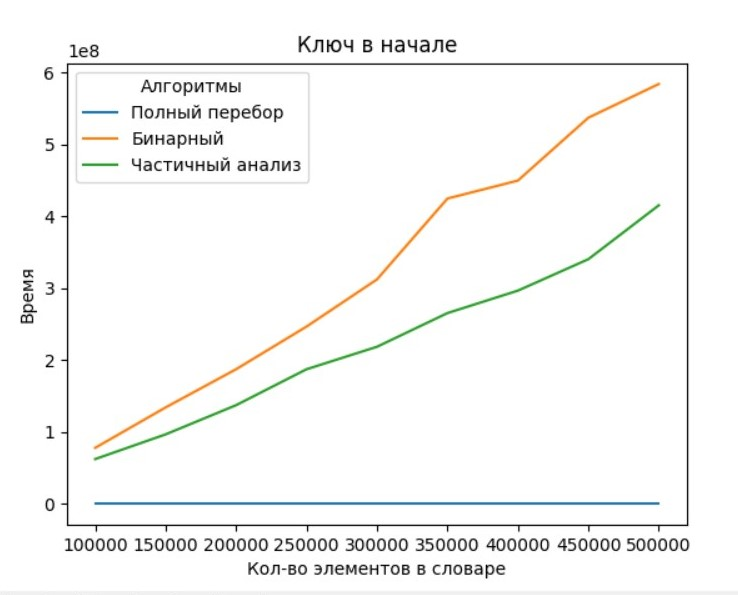
\includegraphics[scale=0.7]{res_start}}
	\caption{График зависимости времени работы от размерности словарей без предварительной сортировки с ключом в начале}
\end{figure}

\newpage
\subsection{Результаты экспериментов для ключа в середине словаря}

\begin{table}[ph!]
  \begin{center}
    \captionsetup{justification=raggedright}
     \caption{Время работы алгоритмов при предварительной сортировке с ключом в середине}
    \label{tab:workcost_classic}
    \begin{tabular}{c|c|c|c}
      \textbf{кол-во пар} & \textbf{t полного перебора (нс)}  & \textbf{t бинарного поиска (нс)} & \textbf{t частичного анализа (нс)}\\
	100000 & 3125000 & 0 & 0\\ 
	150000 & 3125000 & 0 & 0\\ 
	200000 & 3125000 & 0 & 0\\ 
	250000 & 12500000 & 0 & 0\\
	300000 & 9375000 & 0 & 0\\
	350000 & 9375000 & 0 & 0\\
	400000 & 12500000 & 0 & 3125000\\
	450000 & 12500000 & 0 & 3125000\\
	500000 & 12500000 & 0 & 6250000\\
      \hline	
    \end{tabular}
  \end{center}
\end{table}

\begin{figure}[ph!]
	\center{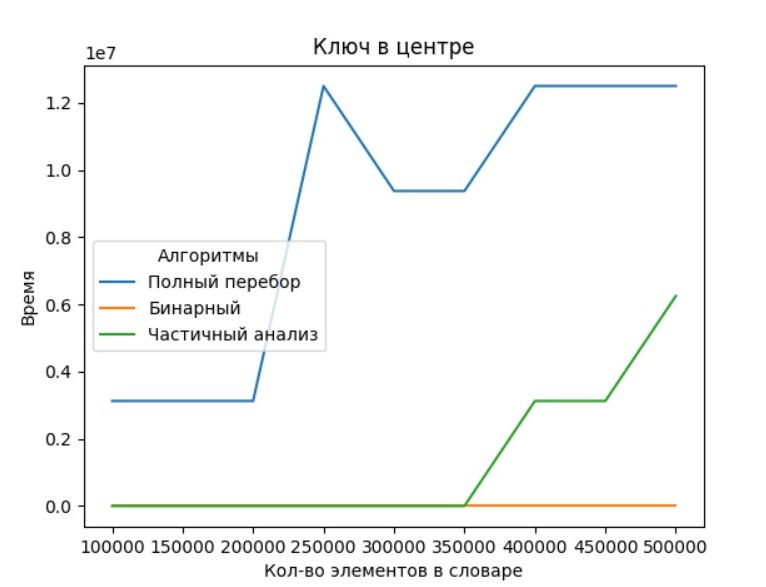
\includegraphics[scale=0.7]{res_center_presort}}
	\caption{График зависимости времени работы от размерности словарей при предварительной сортировке с ключом в середине}
\end{figure}

\newpage
\begin{table}[ph!]
  \begin{center}
    \captionsetup{justification=raggedright}
     \caption{Время работы алгоритмов без предварительной сортировки с ключом в середине}
    \label{tab:workcost_classic}
    \begin{tabular}{c|c|c|c}
      \textbf{кол-во пар} & \textbf{t полного перебора (нс)}  & \textbf{t бинарного поиска (нс)} & \textbf{t частичного анализа (нс)}\\
	100000 & 0 & 81250000 & 62500000\\
	150000 & 3125000 & 131250000 & 96875000\\
	200000 & 6250000 & 187500000 & 150000000\\
	250000 & 9375000 & 259375000 & 193750000\\
	300000 & 9375000 & 337500000 & 225000000\\
	350000 & 9375000 & 381250000 & 259375000\\
	400000 & 9375000 & 437500000 & 300000000\\
	450000 & 12500000 & 534375000 & 359375000\\
	500000 & 12500000 & 578125000 & 412500000\\
      \hline	
    \end{tabular}
  \end{center}
\end{table}

\begin{figure}[ph!]
	\center{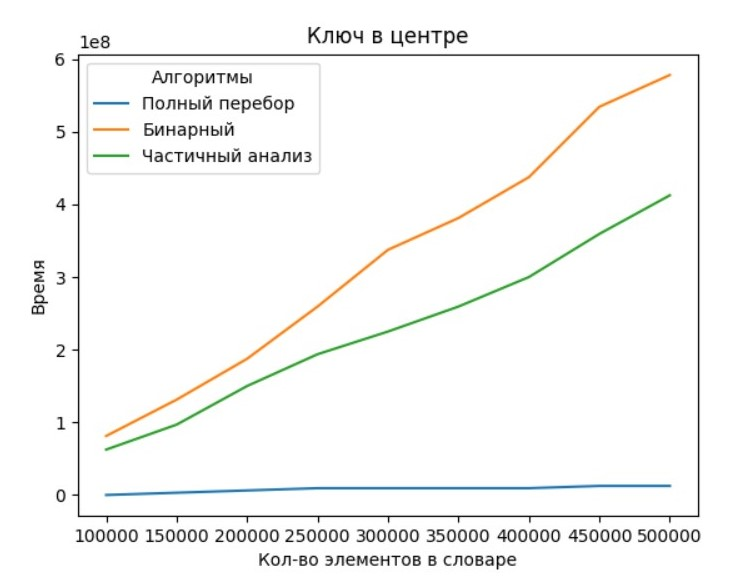
\includegraphics[scale=0.7]{res_center}}
	\caption{График зависимости времени работы от размерности словарей без предварительной сортировки с ключом в середине}
\end{figure}

\newpage
\subsection{Результаты экспериментов для ключа в конце словаря}

\begin{table}[ph!]
  \begin{center}
    \captionsetup{justification=raggedright}
     \caption{Время работы алгоритмов при предварительной сортировке с ключом в конце}
    \label{tab:workcost_classic}
    \begin{tabular}{c|c|c|c}
      \textbf{кол-во пар} & \textbf{t полного перебора (нс)}  & \textbf{t бинарного поиска (нс)} & \textbf{t частичного анализа (нс)}\\
	100000 & 6250000 & 0 & 3125000\\
	150000 & 6250000 & 0 & 0\\
	200000 & 9375000 & 0 & 0\\
	250000 & 18750000 & 0 & 3125000\\
	300000 & 15625000 & 0 & 0\\
	350000 & 21875000 & 3125000 & 0\\
	400000 & 25000000 & 0 & 3125000\\
	450000 & 25000000 & 0 & 3125000\\
	500000 & 34375000 & 0 & 3125000\\
      \hline	
    \end{tabular}
  \end{center}
\end{table}

\begin{figure}[ph!]
	\center{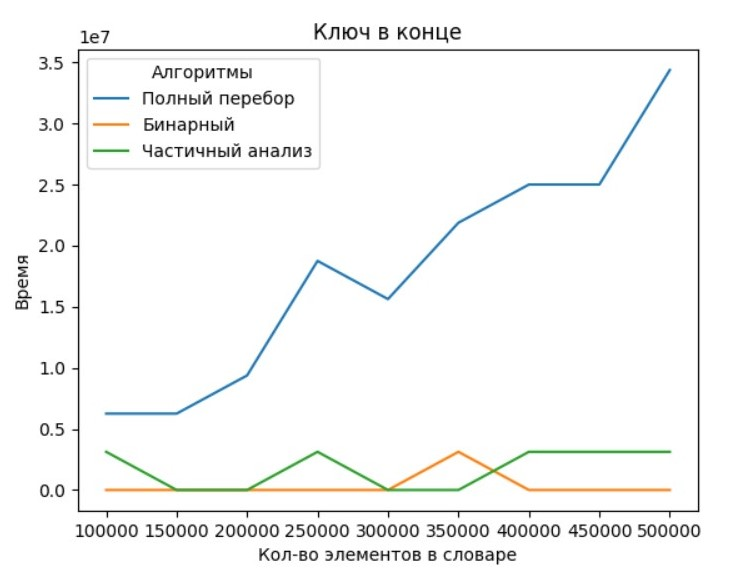
\includegraphics[scale=0.7]{res_end_presort}}
	\caption{График зависимости времени работы от размерности словарей при предварительной сортировке с ключом в конце}
\end{figure}

\newpage
\begin{table}[ph!]
  \begin{center}
    \captionsetup{justification=raggedright}
     \caption{Время работы алгоритмов без предварительной сортировки с ключом в конце}
    \label{tab:workcost_classic}
    \begin{tabular}{c|c|c|c}
      \textbf{кол-во пар} & \textbf{t полного перебора (нс)}  & \textbf{t бинарного поиска (нс)} & \textbf{t частичного анализа (нс)}\\
	100000 & 6250000 & 75000000 & 65625000\\
	150000 & 6250000 & 131250000 & 100000000\\
	200000 & 9375000 & 196875000 & 137500000\\
	250000 & 12500000 & 246875000 & 190625000\\
	300000 & 12500000 & 312500000 & 215625000\\
	350000 & 15625000 & 375000000 & 265625000\\
	400000 & 21875000 & 437500000 & 321875000\\
	450000 & 21875000 & 509375000 & 346875000\\
	500000 & 25000000 & 646875000 & 418750000\\
      \hline	
    \end{tabular}
  \end{center}
\end{table}

\begin{figure}[ph!]
	\center{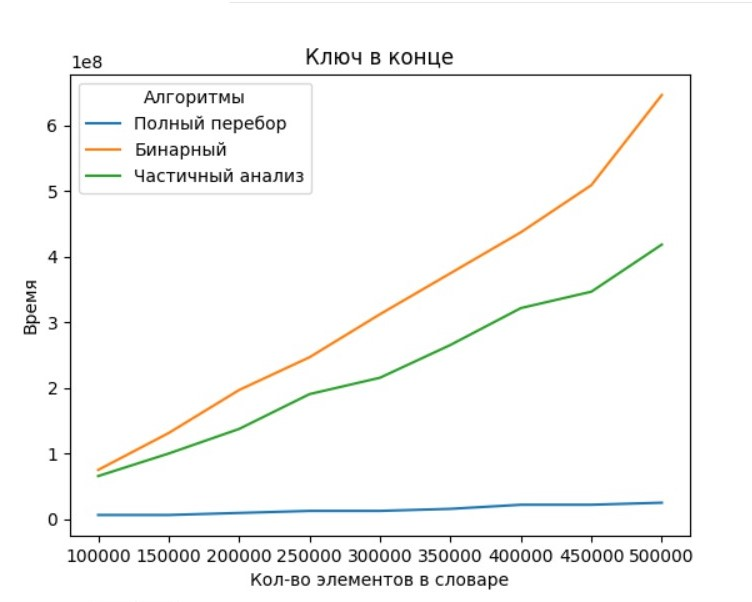
\includegraphics[scale=0.7]{res_end}}
	\caption{График зависимости времени работы от размерности словарей без предварительной сортировки с ключом в конце}
\end{figure}

\newpage
\subsection{Результаты экспериментов для ключа в не из словаря}

\begin{table}[ph!]
  \begin{center}
    \captionsetup{justification=raggedright}
     \caption{Время работы алгоритмов при предварительной сортировке с ключом не из словаря}
    \label{tab:workcost_classic}
    \begin{tabular}{c|c|c|c}
      \textbf{кол-во пар} & \textbf{t полного перебора (нс)}  & \textbf{t бинарного поиска (нс)} & \textbf{t частичного анализа (нс)}\\
	100000 & 6250000 & 0 & 3125000\\
	150000 & 6250000 & 0 & 0\\
	200000 & 9375000 & 0 & 0\\
	250000 & 18750000 & 0 & 3125000\\
	300000 & 15625000 & 0 & 0\\
	350000 & 21875000 & 3125000 & 0\\
	400000 & 25000000 & 0 & 3125000\\
	450000 & 25000000 & 0 & 3125000\\
	500000 & 34375000 & 0 & 3125000\\
      \hline	
    \end{tabular}
  \end{center}
\end{table}

\begin{figure}[ph!]
	\center{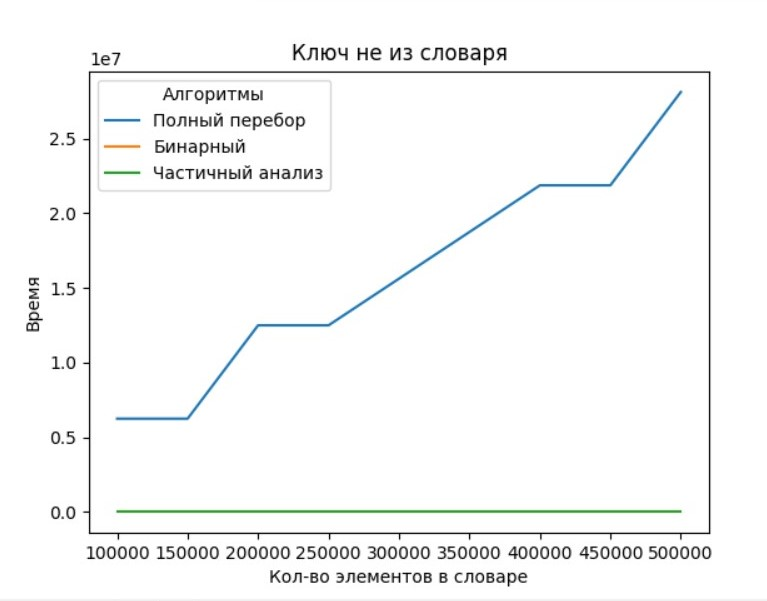
\includegraphics[scale=0.7]{res_none_presort}}
	\caption{График зависимости времени работы от размерности словарей при предварительной сортировке с ключом не из словаря}
\end{figure}

\newpage
\begin{table}[ph!]
  \begin{center}
    \captionsetup{justification=raggedright}
     \caption{Время работы алгоритмов без предварительной сортировки с ключом в начале}
    \label{tab:workcost_classic}
    \begin{tabular}{c|c|c|c}
      \textbf{кол-во пар} & \textbf{t полного перебора (нс)}  & \textbf{t бинарного поиска (нс)} & \textbf{t частичного анализа (нс)}\\
	100000 & 3125000 & 78125000 & 65625000\\
	150000 & 6250000 & 131250000 & 100000000\\
	200000 & 9375000 & 187500000 & 137500000\\
	250000 & 9375000 & 268750000 & 190625000\\
	300000 & 15625000 & 309375000 & 218750000\\
	350000 & 15625000 & 371875000 & 271875000\\
	400000 & 18750000 & 456250000 & 318750000\\
	450000 & 21875000 & 537500000 & 337500000\\
	500000 & 25000000 & 625000000 & 390625000\\
      \hline	
    \end{tabular}
  \end{center}
\end{table}

\begin{figure}[ph!]
	\center{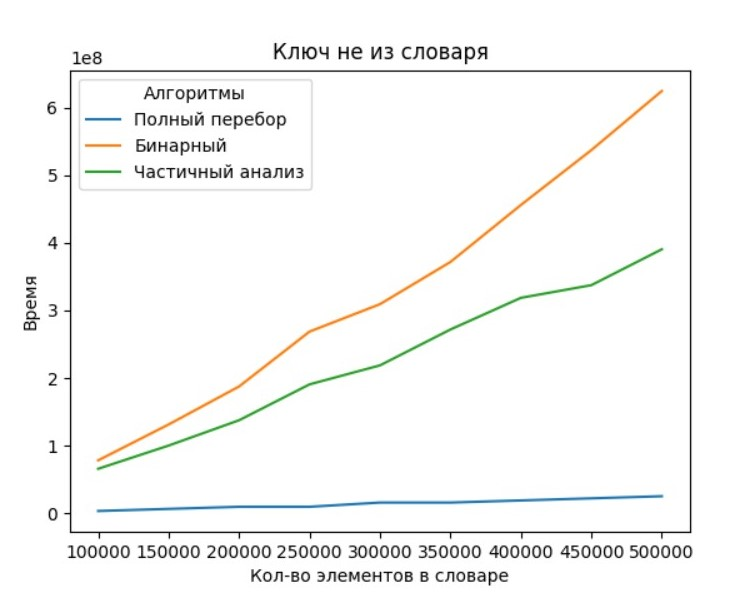
\includegraphics[scale=0.7]{res_none}}
	\caption{График зависимости времени работы от размерности словарей без предварительной сортировки с ключом не из словаря}
\end{figure}

\section{Вывод}
В результате эксперимента было получено, что при предварительной сортировке данных наиболее медленным алгоритмом является алгоритм полного перебора. В случае, когда подготовка исходного массива включается во временные измерения самым быстрым алгоритмом во всех случаях является алгоритм полного перебора, а самым медленным - бинарный поиск. 